\chapter{Raspberry Pi}

Over the course of this semester we will be building a variety of medical and biological sensors.  We will be using the Raspberry Pi as our microcomputer to control them, because of its ease of use, large number of IO pins, and tons of example code to build on.  In this lab we will be introducing the Raspberry Pi and how to use it.  I am going to try to do most things in Python, due to its simplicity and extensibility, but I can't guarantee we won't have to do a little programming in another language.

%All of our Raspberry Pi's have been set up for us by Ken Ulibari, so we all owe him a big thanks for the great job he did.  Should you ever need to install a Raspberry Pi of your own, or modify one of these, my short notes and commands examples are in Appendix~\ref{chapter:RPiRef}.
One thing I really want to bring to your attention is the use of \textbf{git}.  Git is a version control system (VCS), that was designed by Linus Torvalds to handle the development of Linux.  I will be maintaining a git repo at github, which means you will be able to clone it and do a pull any time you want to update it.  You do not have to use git, it just saves time and is a good skill to know for industry.

\section{GIT}

\CommandLine{mkdir code}

\CommandLine{cd  code}

\CommandLine{git clone \url{https://github.com/BaylorBMEELC4372BioInstrumentation/labs.git}}

\CommandLine{cd labs}

\CommandLine{ls}

To update from the main repository, just do a pull

\CommandLine{git pull}

More sample code can be found by:

\CommandLine{cd ~/code}

\CommandLine{git clone \url{http://github.com/adafruit/Adafruit-Raspberry-Pi-Python-Code.git}}

\CommandLine{cd Adafruit-Raspberry-Pi-Python-Code}


\section{Das Blinken LED}

\begin{itemize}
  \item Raspberry Pi (with keyboard, mouse, monitor, cobbler, and breadboard)
  \item 220$\Omega$ - 330$\Omega$ Resistor
  \item LED
\end{itemize}

First you need to assemble the circuit.  Hook up a wire from a gpio pin to the anode (long leg) of the diode, then connect the resistor to ground.  The resistor limits the current flow.  The Pi will output 3.3V and the diode will cause about a .7V drop resulting in a 2.6V drop left over.  The remaining 2.6V flowing through around 220$\Omega$ to 330$\Omega$ will result in around 10mV, which is enough to light the LED but not cause problems sinking or sourcing the current for the Pi.  Generally be careful with more than 20mV - 30mV for an IC.

Boot the Pi by plugging it in.  When the desktop appears, launch a terminal either from the menu or the terminal button.  Type the following line to edit the code to turn on and off with a timer.

\CommandLine{sudo nano \url{das_blinken_light.py}}

Note that nano is a small editor, hence the cute name.  You are welcome to use any editor you like.  You should see something that looks like Code~\ref{code:dbli}.  The only thing you have to edit is the gpio pin number to match the one you used, see Figure~\ref{fig:RPiGPIO}.

\begin{figure}\begin{center}
\caption{Raspberry Pi 2 General Purpose Input Output (GPIO) pinout.}\label{fig:RPiGPIO}
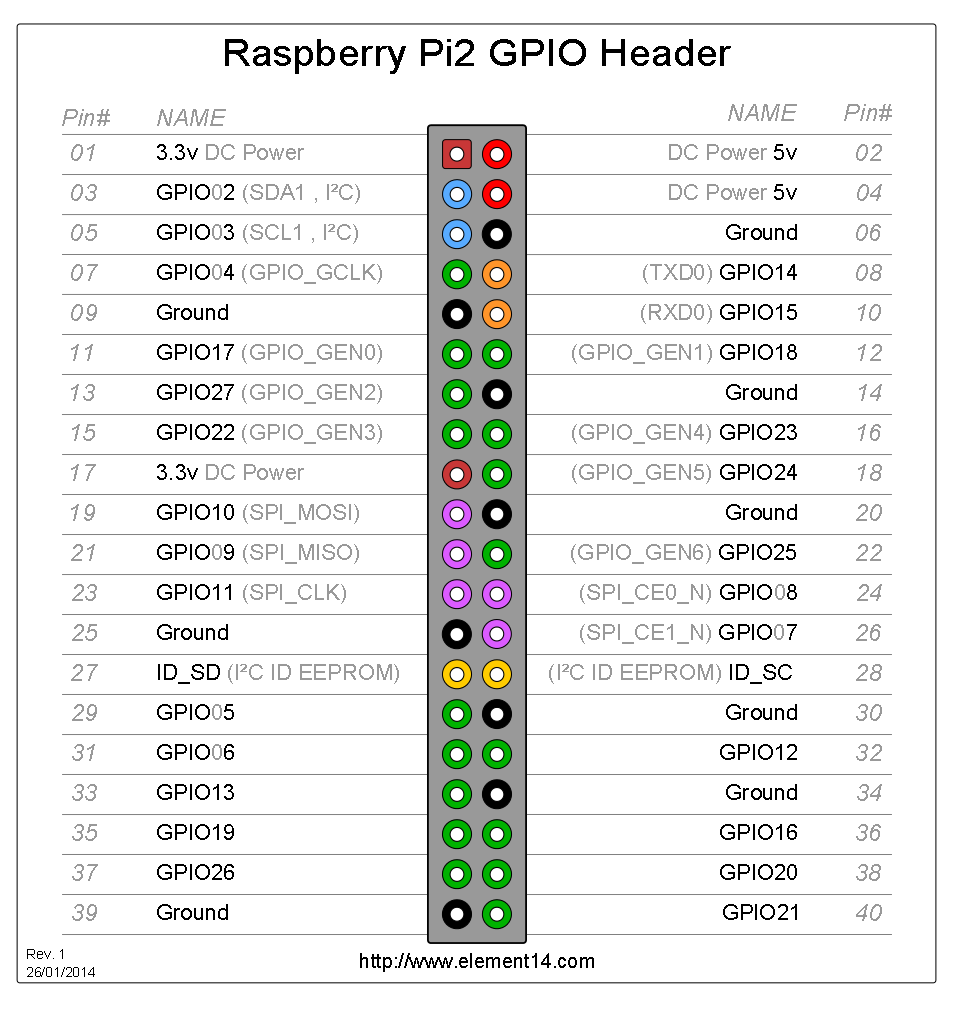
\includegraphics[width=.7\textwidth]{../images/GPIO_Pi2.png}
\end{center}\end{figure}

\Code{Blink the Light.}{code:dbli}{../labs/lab_01/das_blinken_light.py}{Python}

To run the code you need to type the following in the terminal window.

\CommandLine{sudo python \url{das_blinken_light.py}}

You need sudo to give enough permission to access the gpio pins.  The LED should blink on for a sec and off for a sec.

\section{Das Blinken LED II}

\begin{itemize}
  \item all the previous parts
  \item switch
\end{itemize}

Hook up with switch or button to ground.  The Broadcom chip that runs the gpio for the Pi has the ability to connect a pullup or pulldown resistor to an input.  We will thus use a pullup resistor, and the button will pull it down to ground when pressed.

We will now write code to read input and blink led if the button isn't pressed.  Type in:

\CommandLine{sudo nano \url{das_blinken_light_II.py}}

You can also refer to the GitHub repository, if need be.

\Code{Blink the Light while the button is not pressed.}{code:dblii}{../labs/lab_01/das_blinken_light_II.py}{Python}

\CommandLine{sudo python \url{das_blinken_light_II.py}}


\section{Das Blinken LED III}

One last thing for today is to dim the led.  The Raspberry Pi does not have an A/D converter, so we will just deal with two levels based on the button.  We also only have one pulse width modulated output on Broadcom (BCM) pin 18, which is Board pin 12.  Lack of A/D converters is one of several reasons it is not a replacement for a micro-controller, the main one being it doesn't have a real time operating system (RTOS) and lacks the necessary timers, like watchdog timers, to build one.  If you ever need a micro-controller then use an Ardino, MSP430, or similar.  The Pi has a bunch of advantages too in standard tools, quad core, and so on.  We care more about the later for labs and testing.  If you ever build patient used tools, get a micro-controller as you need the RTOS.

Getting back to the point, we want to have the LED on all the time now, and we will dim it when the button is pushed.  To handle the diming, we will use a pulse width modulator.  We will set the frequency to 50Hz, which is a reasonable refresh rate, and will use the duty cycle (percent of the wave that is high) to control the brightness.  This is a simple and standard way to handle this.  Type in:

\CommandLine{sudo nano \url{das_blinken_light_III.py}}

You can also refer to the GitHub repository, if need be.

\Code{Dim the Light while the button is pressed.}{code:dbliii}{../labs/lab_01/das_blinken_light_III.py}{Python}

\CommandLine{sudo python \url{das_blinken_light_III.py}}

